\documentclass[10pt]{beamer}

% Konfigurasi Tema
\usetheme{Madrid}
\usecolortheme{whale}

% Paket Tambahan
\usepackage[utf8]{inputenc}
\usepackage[T1]{fontenc}
\usepackage{amsmath}
\usepackage{graphicx}
\usepackage{amssymb}
\usepackage{tikz}
\usetikzlibrary{shapes,arrows}

% Meta Data Presentasi
\title[Bedah Konsep VQE]{Semua Konsep yang Ada di Algoritma VQE untuk Optimisasi Portofolio}
\date{\today}

\begin{document}

% --- SLIDE 1: JUDUL ---
\begin{frame}
    \titlepage
\end{frame}

% --- SLIDE 2: DAFTAR ISI ---
\begin{frame}{Outline Pembahasan}
    \tableofcontents
\end{frame}

% ==========================================
% BAGIAN 1: FORMULASI MASALAH
% ==========================================
\section{Formulasi Masalah: Matematika ke Fisika}

% --- SLIDE 3: MODEL MATEMATIKA ---
\begin{frame}{Model Matematika Portofolio (MPT)}
    \textbf{Dua Kekuatan yang Saling Tarik-Menarik:}
    \begin{enumerate}
        \item \textbf{Return ($\mu$):} Keuntungan rata-rata (Linear). \textit{Ingin Dimaksimalkan.}
        \item \textbf{Risiko ($\sigma$):} Matriks kovariansi antar aset (Kuadratik). \textit{Ingin Diminimalkan.}
    \end{enumerate}
    
    \vspace{0.5cm}
    \textbf{Persamaan Penyeimbang:}
    \[ C' = \underbrace{-\lambda(\text{Return})}_{\text{Tarik ke Atas}} + \underbrace{(1-\lambda)(\text{Risiko})}_{\text{Tarik ke Bawah}} \]
    
    \vspace{0.2cm}
    \begin{alertblock}{Visualisasi Konsep}
        \centering
        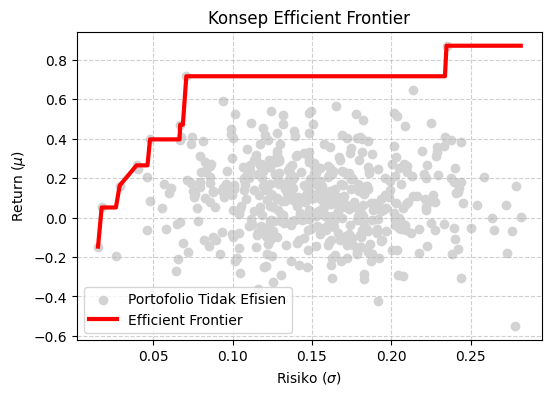
\includegraphics[width=0.25\textwidth]{Efficient_Frontier.png}
    \end{alertblock}
\end{frame}

% --- SLIDE 4: QUBO ---
\begin{frame}{QUBO sebagai Jembatan Matematika ke Kuantum}
    \textbf{Q.U.B.O:} \textit{Quadratic Unconstrained Binary Optimization}
    
    \begin{itemize}
        \item \textbf{Quadratic:} Karena adanya interaksi risiko antar saham ($\sigma_{ij} x_i x_j$).
        \item \textbf{Binary:} Keputusan tegas: $1$ (Beli) atau $0$ (Tidak).
        \item \textbf{Unconstrained:} Batasan "Budget" diubah menjadi \textbf{Penalti}.
        \item \textbf{NP-Hard:} Kompleksitas meledak secara eksponensial seiring bertambahnya aset.
    \end{itemize}

    \vspace{0.3cm}
    \begin{block}{Konsep "Sumur Penalti" (Penalty Well)}
        \centering
        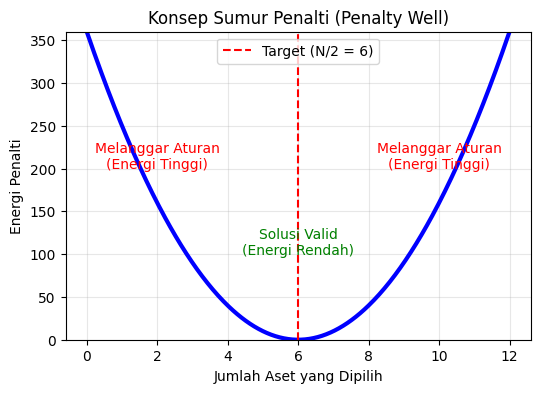
\includegraphics[width=0.25\textwidth]{Sumur_Penalti.png}
    \end{block}
\end{frame}

% --- SLIDE BARU: IMPLEMENTASI HAMILTONIAN ---
\begin{frame}{Implementasi: Transformasi ke Hamiltonian Ising}
    \textbf{1. Mapping Variabel (Dari Keuangan ke Fisika):}
    \[ x_i \in \{0,1\} \xrightarrow{\text{Transformasi}} s_i \in \{+1,-1\} \xrightarrow{\text{Operator}} \hat{Z}_i \]
    \begin{itemize}
        \item Variabel biner $x_i$ (Beli/Tidak) diubah menjadi operator Pauli-Z.
    \end{itemize}
    
    \vspace{0.3cm}
    \textbf{2. Konstruksi Hamiltonian ($\hat{H}$):}
    Masalah optimisasi dikemas dalam satu persamaan energi total:
    \[ \hat{H} = \underbrace{-\sum h_i \hat{Z}_i}_{\text{Bias Linear (Return)}} - \underbrace{\sum J_{ij} \hat{Z}_i \hat{Z}_j}_{\text{Interaksi (Risiko)}} \]
    
    \vspace{0.2cm}
    \begin{block}{Interpretasi Parameter}
        \begin{itemize}
            \item \textbf{$h_i$:} Mengandung informasi \textit{Expected Return} dan suku linear penalti.
            \item \textbf{$J_{ij}$:} Mengandung informasi \textit{Covariance Matrix} dan interaksi penalti.
            \item \textbf{Tujuan:} $\min \langle \psi | \hat{H} | \psi \rangle \equiv$ Profit Maksimal \& Risiko Minimal.
        \end{itemize}
    \end{block}
\end{frame}

% ==========================================
% BAGIAN 2: KOMPONEN KUANTUM
% ==========================================
\section{Komponen Sirkuit Kuantum}

% --- SLIDE 5: VQE \& ANSATZ ---
\begin{frame}{VQE dan Peran Ansatz}
    \textbf{Variational Quantum Eigensolver (VQE)} adalah algoritma hibrida.
    
    \vspace{0.5cm}
    \begin{itemize}
        \item \textbf{VQE Loop:} Mencari energi terendah (\textit{ground state}) secara iteratif.
        \item \textbf{Ansatz ($\mid \psi(\theta) \rangle$):} 
        \begin{itemize}
            \item Secara harfiah berarti "Tebakan Awal".
            \item Adalah kerangka sirkuit kuantum dengan parameter yang bisa diubah-ubah.
        \end{itemize}
        \item \textbf{Parameter $\theta$:} "Knob" atau tombol putar yang dikendalikan komputer klasik untuk membentuk fungsi gelombang terbaik.
    \end{itemize}
\end{frame}

% --- SLIDE 6: TWO-LOCAL ANSATZ ---
\begin{frame}{Ansatz 1: Two-Local (Struktur Standar)}
    \begin{columns}
        \column{0.5\textwidth}
        \textbf{Karakteristik:}
        \begin{itemize}
            \item Struktur berlapis (\textit{Layered}).
            \item Sangat umum di era NISQ.
        \end{itemize}
        
        \vspace{0.3cm}
        \textbf{Komponen:}
        \begin{itemize}
            \item \textbf{Rotasi ($R_y, R_z$):} Eksplorasi superposisi individu.
            \item \textbf{Entanglement ($CNOT$):} Mensimulasikan korelasi antar aset.
        \end{itemize}
        
        \column{0.5\textwidth}
        \begin{exampleblock}{Diagram Sirkuit}
            \centering
            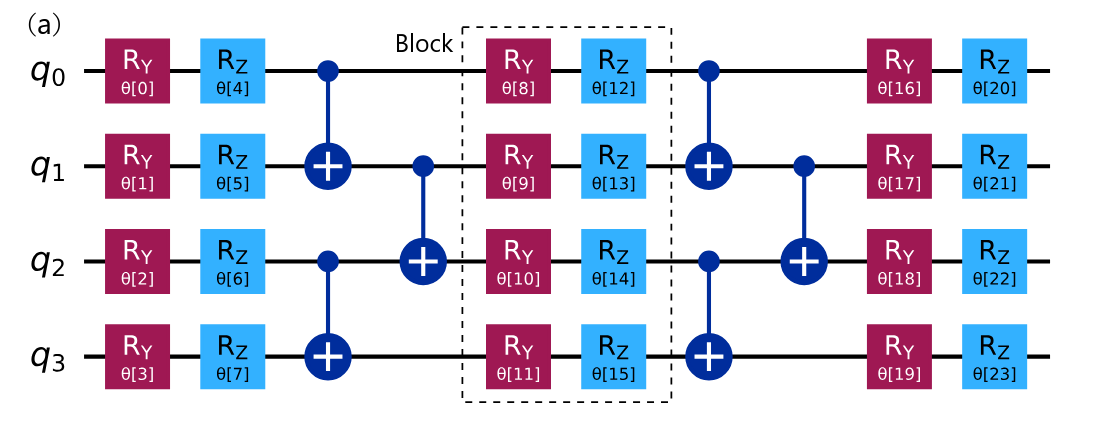
\includegraphics[width=\textwidth]{Gambar_1a.png}
        \end{exampleblock}
    \end{columns}
\end{frame}

% --- SLIDE 7: BLOCK ANSATZ ---
\begin{frame}{Ansatz 2: Block Ansatz (Struktur Modular)}
    \begin{columns}
        \column{0.5\textwidth}
        \textbf{Karakteristik:}
        \begin{itemize}
            \item Berbasis modul fungsional (\textit{Block-based}).
            \item Qubit diproses intensif dalam satu blok sebelum lanjut.
        \end{itemize}
        
        \vspace{0.3cm}
        \textbf{Kelebihan:}
        \begin{itemize}
            \item Menciptakan keterbelitan yang lebih dalam (\textit{deeper entanglement}).
            \item Operasi \textit{controlled-unitary} yang fleksibel.
        \end{itemize}
        
        \column{0.5\textwidth}
        \begin{exampleblock}{Diagram Sirkuit}
            \centering
            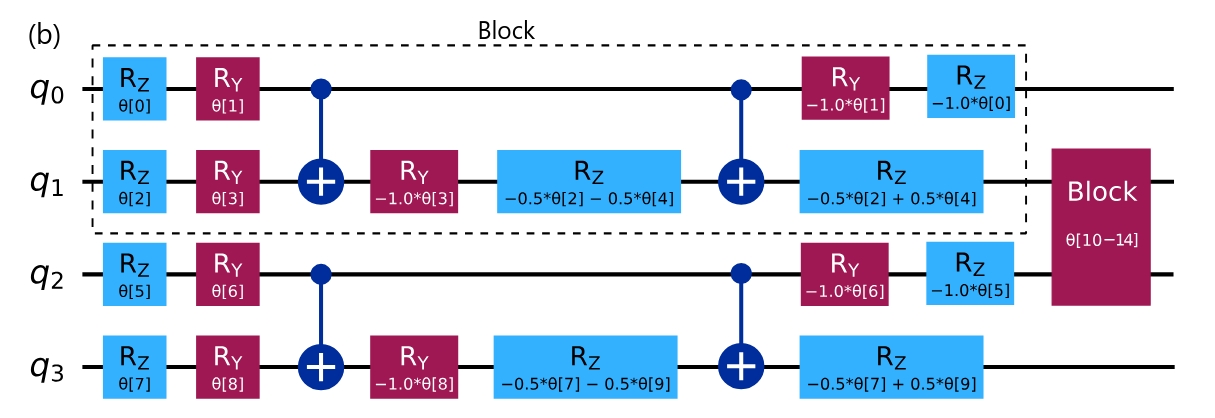
\includegraphics[width=\textwidth]{Gambar_1b.png}
        \end{exampleblock}
    \end{columns}
\end{frame}

% ==========================================
% BAGIAN 3: FUNGSI BIAYA (COST FUNCTION)
% ==========================================
\section{Inovasi Fungsi Biaya}

% --- SLIDE 8: MEAN VS CVAR ---
\begin{frame}{CVaR}
    \textbf{Mengapa "Rata-rata Energi" itu kurang?}
    \begin{itemize}
        \item \textbf{Expectation Value (Mean):} Merata-ratakan seluruh hasil sampling. Solusi "emas" (langka) sering tertutup oleh solusi "sampah" (banyak).
    \end{itemize}
    
    \vspace{0.5cm}
    \textbf{Solusi: CVaR (Conditional Value-at-Risk)}
    \begin{itemize}
        \item Hanya mengambil rata-rata dari \textbf{Ekor Distribusi} ($\alpha\%$ terendah).
        \item \textbf{Logika:} "Fokus hanya pada kandidat juara, abaikan sisanya."
    \end{itemize}
    
    \vspace{0.3cm}
    \begin{alertblock}{Distribusi Energi}
        \centering
        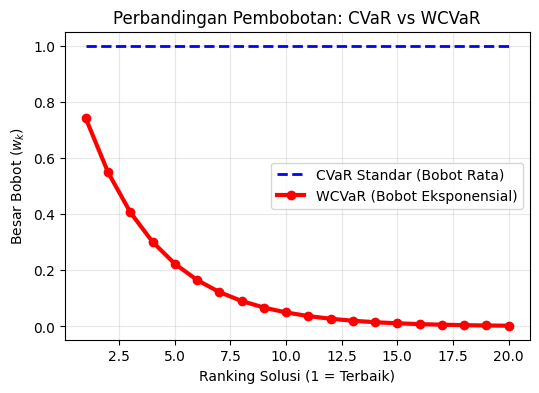
\includegraphics[width=0.25\textwidth]{Perbandingan_Bobot_WCVaR.png}
    \end{alertblock}
\end{frame}

% --- SLIDE 9: WCVAR ---
\begin{frame}{Weighted CVaR (WCVaR)}
    \textbf{Kelemahan CVaR Biasa:}
    \begin{itemize}
        \item Memberi bobot SAMA pada Juara 1 dan Juara Terakhir dalam daftar top $\alpha$.
    \end{itemize}
    
    \vspace{0.3cm}
    \textbf{Penyempurnaan WCVaR:}
    \begin{itemize}
        \item Memberi bobot \textbf{BERBEDA} berdasarkan \textbf{Ranking}.
        \item \textbf{Rumus Bobot:} $w_k = \exp(-\beta k)$
        \item \textbf{Efek:} Memberi sinyal sangat kuat ("Hadiah Besar") ke optimizer jika menemukan solusi ranking 1.
    \end{itemize}
    
    \vspace{0.3cm}
    \begin{block}{Kurva Bobot}
        \centering
        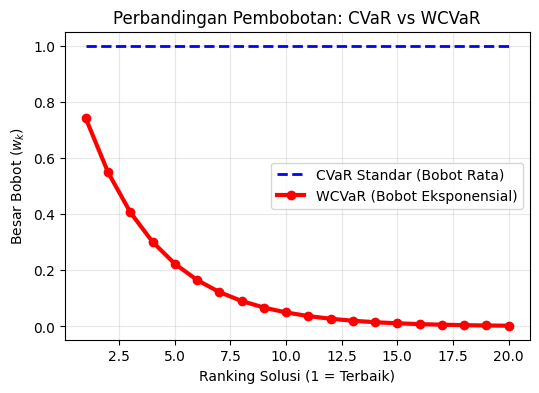
\includegraphics[width=0.25\textwidth]{Perbandingan_Bobot_WCVaR.png}
    \end{block}
\end{frame}

% ==========================================
% BAGIAN 4: OPTIMIZER KLASIK
% ==========================================
\section{Optimizer Klasik}

% --- SLIDE 10: COBYLA VS CMA-ES ---
\begin{frame}{COBYLA vs CMA-ES}
    \begin{columns}
        \column{0.5\textwidth}
        \textbf{COBYLA (Standar)}
        \begin{itemize}
            \item \textit{Constrained Optimization BY Linear Approximation}.
            \item Sering terjebak di \textit{Local Minima} (lembah palsu).
            \item Kurang tahan terhadap \textit{noise}.
        \end{itemize}
        
        \column{0.5\textwidth}
        \textbf{CMA-ES (Pilihan Paper)}
        \begin{itemize}
            \item \textit{Covariance Matrix Adaptation Evolution Strategy}.
            \item \textbf{Evolutionary:} Menggunakan populasi (banyak agen), bukan satu agen.
            \item \textbf{Derivative-Free:} Cocok untuk WCVaR yang kasar.
        \end{itemize}
    \end{columns}
    
    \vspace{0.5cm}
    \begin{exampleblock}{Visualisasi CMA-ES}
        \centering
        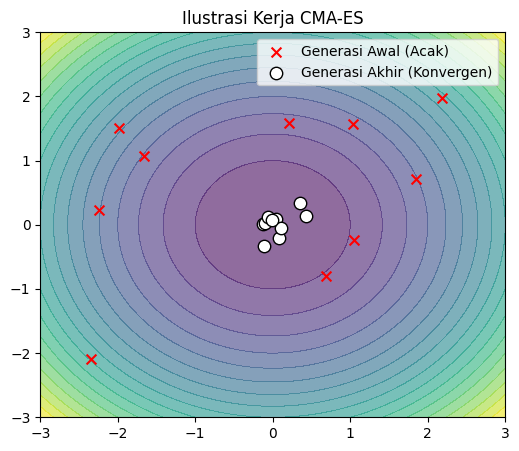
\includegraphics[width=0.25\textwidth]{Ilustrasi_CMA_ES.png}
    \end{exampleblock}
\end{frame}

% ==========================================
% BAGIAN 5: KESIMPULAN
% ==========================================
\section{Kesimpulan Integrasi}

% --- SLIDE 11: THE BIG PICTURE ---
\begin{frame}{Alur Kerja Lengkap}
    \begin{enumerate}
        \item \textbf{QUBO:} Masalah Keuangan diterjemahkan ke Fisika (Hamiltonian).
        \vspace{0.3cm}
        \item \textbf{Ansatz:} Membentuk kandidat solusi (Sirkuit Kuantum).
        \vspace{0.3cm}
        \item \textbf{WCVaR:} Menilai kualitas solusi (Fungsi Biaya Selektif \& Berbobot).
        \vspace{0.3cm}
        \item \textbf{CMA-ES:} Mengarahkan pencarian parameter berdasarkan nilai WCVaR agar semakin mendekati solusi optimal.
    \end{enumerate}
    
    \vspace{0.5cm}
    \centering
    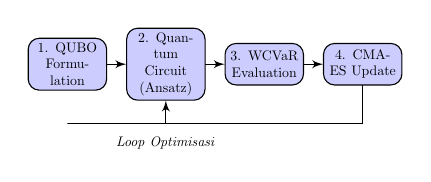
\begin{tikzpicture}[scale=0.5, transform shape, node distance=1.5cm, auto]
        % Styles
        \tikzstyle{block} = [rectangle, draw, fill=blue!20, text width=5em, text centered, rounded corners, minimum height=3em]
        \tikzstyle{line} = [draw, -latex']
        \tikzstyle{cloud} = [draw, ellipse, fill=red!20, node distance=3cm, minimum height=2em]

        % Nodes
        \node [block] (qubo) {1. QUBO Formulation};
        \node [block, right of=qubo, node distance=2.5cm] (ansatz) {2. Quantum Circuit (Ansatz)};
        \node [block, right of=ansatz, node distance=2.5cm] (wcvar) {3. WCVaR Evaluation};
        \node [block, right of=wcvar, node distance=2.5cm] (cmaes) {4. CMA-ES Update};
        
        % Edges
        \path [line] (qubo) -- (ansatz);
        \path [line] (ansatz) -- (wcvar);
        \path [line] (wcvar) -- (cmaes);
        \path [line] (cmaes) |- (0,-1.5) -| (ansatz); % Loop feedback
        
        % Labels
        \node [below of=ansatz, node distance=2cm] (loop_label) {\textit{Loop Optimisasi}};
    \end{tikzpicture}
    
    \vspace{0.2cm}
    \textbf{Hasil:} Probabilitas tinggi menemukan portofolio optimal di era NISQ.
\end{frame}

\end{document}
